\chapter{Překlad obrázkových popisků}
\label{chap:preklad}

Popisky obrázků v datasetu Profimedie jsou v angličtině. Jedním z cílů aplikace je poskytnout kromě angličtiny vyhledávání i v jiném jazyce. Zaměřujeme se na češtinu, ale podobné úvahy a postupy platí většinou i pro jiné jazyky. Jsou v podstatě dvě možnosti, jak implementovat vyhledávání v češtině. Můžeme buď překládat do angličtiny hledané texty a klíčová slova, nebo předpřeložit dataset Profimedie.

My jsme se rozhodli pro druhou možnost. Musíme tedy přeložit všechny texty v datasetu Profimedie. Vzhledem k tomu, že obrázků je více než 20 milionů, nepřipadá lidský překlad v úvahu z časových i finančních důvodů. Jedinou reálnou možností je použít překlad strojový.

\section{Strojový překlad}

Strojový překlad jako obor zažívá velký rozvoj. Potřeba překladu stále celosvětově prudce stoupá. To jednak zvyšuje poptávku po kvalitním strojovém překladu a dále to strojovému překladu dává k dispozici velké množství lidských překladů, které jsou pro kvalitní strojový překlad nezbytné. Lze brát v úvahu i pravidlové překladové systémy, které ke své práci tolik dat většinou nepotřebují. Obecnější a pro většinu jazykových párů nejlepší řešení však nabízí frázový statistický strojový překlad.

\section{Frázový statistický strojový překlad}

 Frázový statistický strojový překlad\cite{koehn} ke své práci potřebuje databázi lidsky přeložených frází. Fráze jsou několikaslovné kusy přeloženého textu. Typicky se získávají z paralelního korpusu textů ve zdrojovém a cílovém jazyce. Soubor s frázovými daty obsahuje položku s textem fráze ve zdrojovém a cílovém jazyce spolu s pravděpodobností, že je takový překlad fráze správný.

Druhým důležitým vstupem strojového frázového systému je korpus cílového jazyka, ze kterého se vytvoří jazykový model. Slouží zejména k tomu, aby k sobě poskládané fráze v cílovém jazyce dobře \uv{seděly}. Pokud máme překladový i jazykový model, můžeme vyjádřit pravděpodobnost překladu pomocí základního vzorce statistického strojového překladu. Překládáme řetězec $f$ ve zdrojovém jazyce. K dispozici máme překladový model $p(f|e)$, který udává pravděpodobnost toho, že řetězec $f$ ve zdrojovém jazyce je překladem řetězce $e$ v cílovém jazyce. Jazykový model $p(e)$ nám vrací pravděpodobnost řetězce $e$ v cílovém jazyce. Chceme získat takový řetězec $\tilde{e}$, pro který je pravděpodobnost $p(e|f)$ nevyšší. Pomocí Bayesova pravidla můžeme k hledání takové fráze použít překladový a jazykový model:

\begin{equation}
 \tilde{e} = arg \max_{e \in e^*} p(e|f) = arg \max_{e\in e^*} p(f|e) p(e) 
\end{equation}

V praxi je potřeba u kvalitního strojového překladu vyřešit mnoho dalších problémů. K lepším výsledkům překladu potřebujeme reordering model, který umožňuje přesouvat pozice frází mezi zdrojovým a cílovým textem. 

Dobrý frázový překlad potřebuje ke svému chodu miliony frází. Vyhledávání nejpravděpodobnějšího překladu v takovém množství dat je náročná úloha. Algoritmy, které umožňují vyhledávat ve velkém množství překladových dat jsou implementována v knihovně Moses\cite{moses}, která je dostupná pod volnou licencí včetně základních překladových modelů pro některé jazykové páry.

\section{Charakteristika dat pro překlad}

Pro správné fungování vyhledávání v českém jazyce je potřeba přeložit klíčová slova v Profimedia datech do češtiny. Slova v korpusu jsou oddělena mezerou. Je ale zřejmé, že některá slova vedle sebe k sobě patří --- jsou to fráze --- zatímco některá nikoliv. Naskytují se tedy zhruba tři možnosti, jak takový text přeložit.


\section{Překlad vět}

\begin{figure}[h]
  \centering
  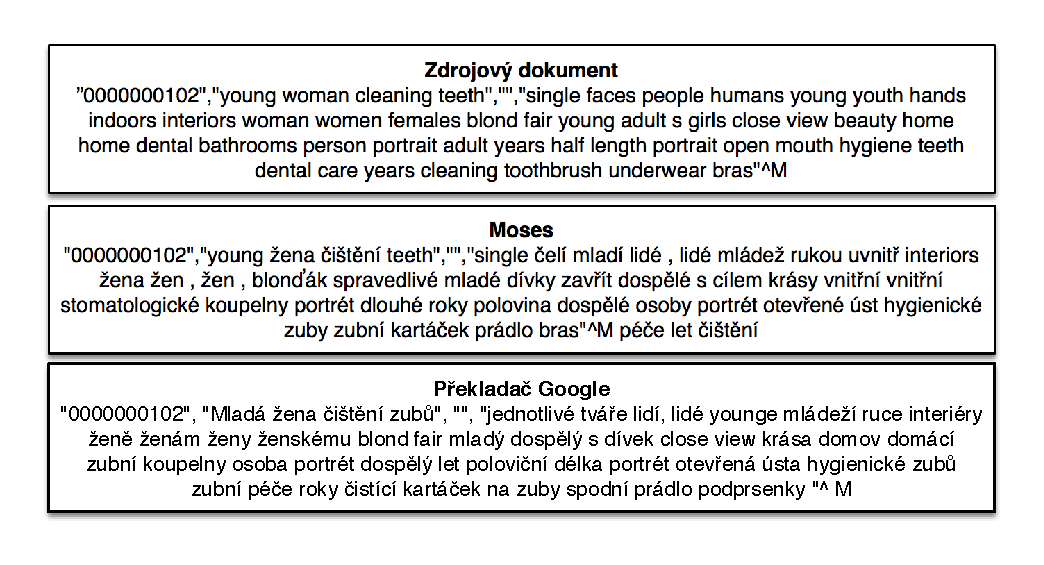
\includegraphics[width=150mm]{translate.eps}
  \caption{Ukázka překladu metadat k obrázku pomocí Mosese a Překladače Google.}
  \label{fig:translate}
\end{figure}

První možností je přistupovat k souboru klíčových slov u každého obrázku jako k větě a použít frázový strojový překlad --- buď Moses, nebo Překladač Google\cite{googletranslate} --- k překladu z angličtiny do češtiny. Tento přístup má několik problémů. Frázový překlad se snaží aplikovat fráze z překladového modelu. V našem souboru klíčových slov ale mohou být vedle sebe slova, která tvoří frázi pouze zdánlivě. Například můžeme mít fotku dítěte, které stojí před automobilem značky Seat se dvěma klíčovými slovy vedle sebe --- \uv{child} a \uv{seat}. Frázový překlad z angličtiny do češtiny pochopí tato dvě slova jako fráze, které do češtiny přeloží frází \uv{dětské sedadlo}, která ovšem neodpovídá popisku obrázku.

Dalším problémem tohoto přístupu je časová a finanční náročnost takového řešení. Frázový překlad je dosti náročný algoritmus a překlad dvaceti milionů vět může být dosti obtížný. Překlad pomocí Mosese nás omezuje výpočetní složitostí. Na jednom stroji by takový překlad trval řádově několik dní. Pokud bychom k překladu 20 milionů vět použili Překladač Google, jsme zase omezení cenou za přístup k překladovému API společnosti Google.

Pro práci s Mosesem jsme zvolili překladový a jazykový model pro překlad z angličtiny do češtiny, které jsou poskytnuty přímo s Mosesem ve verzi XX. Obrázek \ref{fig:translate} porovnává překlad metadat k jednomu z obrázků datasetu Profimedie v Mosesovi s distribuovanými překladovými daty s překladem pomocí Překladače Google. Je vidět, že Překladač Google poskytuje kvalitnější překlad. 

\section{Překlad slov}

Jednodušším přístupem k překladu klíčových slov je přístup slovníkový, tedy překlad každého slova zvlášť. Nejprve je potřeba ze souboru klíčových slov u všech obrázků vyextrahovat slova. Ty pak lze přeložit přímo s použitím slovníku, nebo pomocí frázového strojového překlad (ten použije jednoslovné fráze) Mosesem, či Překladačem Google. Výhodou oproti předchozímu přístupu je menší množství dat a tedy i nižší finanční a časová náročnost takového překladu. Takový systém překladu ale nedokáže detekovat fráze a kvalita překladu slovo od slova je typicky horší než překlad delších frází. Vezměme si například anglická slova \uv{weather} a \uv{vane}. Slovníkový překlad nám slova přeloží jako \uv{počasí} a \uv{lopatka}. Pokud se ale tato slova nachází vedle sebe, je pravděpodobnějším překladem slovo \uv{korouhvička}.

\section{Překlad frází}

Poslední možností je oba předchozí principy zkombinovat --- nejprve detekovat v souboru klíčových slov fráze a ty pak přeložit statistickým strojovým překladem. Detekci frází z datasetu Profimedia provedl ve své bakalářské práci\cite{botorek} Jan Botorek. Zkoušel detekovat N-gramy v databázi WordNet\cite{wordnet} a Wikipedii. Výsledky této detekce frází lze použít právě ke zlepšení překladu z angličtiny do cizích jazyků. Na slova, která nejsou detekována ve frázi, se použije slovníková metoda. Na překlad detekovaných frází lze použít přímo statistický strojový překlad.


\section{Řešení}

Výsledná aplikace nakonec používá poslední možnost. Bližší informace jsou v Kapitole \ref{chap:implementace}. Slova byly přeloženy pomocí Překladače Google, který překládá s lepšími výsledky než dostupný model pro překladový nástroj Moses.

Překlad frází by ovšem pomocí Překladače Google byl příliš drahý a pomocí Mosese zase příliš pomalý. Použili jsme tedy jednoduchou metodu, která používá pouze překladový model. Fráze z datasetu Profimedia byla přeložena pouze tehdy, když se její překlad nacházel v překladovém modelu. Fráze, které se v překladovém modelu nenacházely, byly přeloženy slovo od slova. Metodou přesné shody s překladovým modelem bylo přeloženo $18\ 006$ z celkového počtu $899\ 244$ detekovaných frází v Profimedia datasetu.

\section{Závěr}

Překlad klíčových slov z korpusu Profimedia není typickou překladovou úlohou --- nepřekládají se celé věty. Přesto je dokonalý výsledek nemožný. I lidští překladatelé s citem pro jazyk by v této překladové úloze dávali rozdílné výsledky. Strojový překlad zdaleka není na takové úrovni, aby dokázal z širšího kontextu vybrat správný překlad. Navíc lidský překladatel může u překladu klíčových slov využít přímo obrázek, ke kterému se klíčová slova vztahují. Může tak z obrázku posoudit, zda má slovo \uv{single} přeložit jako \uv{jednolůžkový}, nebo ve významu \uv{jeden}. Lepší překlad by mohl přinést překladový model natrénovaný na speciálnější množině dat bližší korpusu Profimedie. Vytvořit takový model by ovšem bylo nad rámec této práce.

Navrhovaný mechanismus překladu poskytuje uspokojivý, i když značně nedokonalý, překlad klíčových z angličtiny do češtiny. Jednoduše jde zevšeobecnit i pro překlad do dalších jazyků, pro které máme slovník a překladový model.

